%%%%%%%%%%%%%%%%%%%%%%%%%%%%%%%%%%%%%%%%%%%%%%
\section{Beamline instrumentation}
\label{sec:beaminstruments}

The H4 beamline will be instrumented with a number of beamline detectors to provide information 
 about the beam profile, position, momentum, particle identification, and trigger capability. 
This section discusses the reference design for the beam instrumentation. 
%\fixme{Is `baseline design' the right term to use?}

%%%%%%%%%%%%%%%%%%%%%%%
\subsection{Beam profile monitoring, particle tracking and momentum measurements}

Operation of the beamline requires at least one beam monitor, able to provide the beam profile in two dimensions ({\it x,y}) at the entrance point to the NP04 cryostat.   The beam monitor can also be exploited for data analysis, provided that it delivers data on an event-by-event basis. Another monitor, located immediately downstream of the last bending magnet, is added in the layout  in order to determine the incident particle  direction and position at the front face of the cryostat, and match it with the reconstructed track in the LAr active volume.

%The uncertainty in momentum resolution of the beam can be reduced by measuring the momentum particle by particle, 
To reduce the uncertainty due to the momentum spread of the beam around the central selected value, the momentum can be measured particle by particle
with a set of three detectors placed one upstream and two downstream of the bending magnets B18 (see Figure~\ref{fig:beamoptics}).  
Preliminary results using full simulations indicate that a momentum resolution on the order of  2\% is achievable. 
%
\paragraph{Fiber tracker}
The CERN Beam Instrumentation group is designing and fabricating
 the beam monitors %based on 
 using scintillating fiber technology, where %, which 
 the fibers have a polystyrene core surrounded by cladding. Fibers provide a light yield of $\sim$8000 photons/MeV, deposited with fast rise and decay times of 1--3 ns. The design foresees 1 mm square fibers in two planes to provide $x$ and $y$ coordinates. Fibers will be mirrored on one end to increase
light collection.  Every monitor consisting of two planes of 1~mm thick fibers adds 0.47\% of a radiation length ($X_0$) to the material budget - the amount of material distributed along the beamline and crossed by the beam particles before entering the TPC active volume. 
The three devices for momentum measurement will consist of one layer only, oriented perpendicularly to the magnet deflection.
A fiber plane is made out of 192 fibers with no space between them. It will cover an area of 192~mm $\times$ 192~mm and fits in the beamline.
Scintillation light will be read out using SiPMs.
%
%\fixme{Need to decide on one and describe that one. (Anne : ambiguous sentence; clarify `read out by... depending on...'}
These detectors for position and momentum measurement are 
%designed to work inside the vacuum chamber and can be 
mounted through special flanges along the beam pipe, without the need to break the vacuum.

%\paragraph{Multi-wire proportional chambers}
%As a backup solution,
%Fermilab has multi-wire proportional chambers (MWPCs) with $x-y$ sense plane
%readout, measuring approximately 128~mm $\times$ 128~mm, readily available that can also be used as beam profile monitors.  
%Chambers add 2\% nuclear collision lengths and 7\% radiation lengths.
%\fixme{2\% of a nuclear collision length etc.?}
% These chambers have a long history, so installation, integration and commissioning should be straightforward. They are operated in air, thus would require dividing the beamline vacuum into sections.

%%%%%%%%%%%%%%%%%%%%%%%
\subsection{Particle identification}

The H4 beamline is capable of delivering two types of beams, electron and hadron. % beams. 
While the electron beam is relatively pure, the hadron beam consists of a mixture of electrons, pions, kaons, and protons. Therefore, for the hadron beam, it is essential to have an efficient particle identification system to cleanly tag particle types on a particle-by-particle basis. To achieve this goal, a particle identification system based on a combination of threshold Cherenkov counters and time-of-flight (ToF) system is planned for ProtoDUNE-SP. 
Cherenkov counters can be placed in the last segment of the beamline, between the last bending magnet and the cryostat. 
%Space for a ToF system is available, provided that the detector envelope along the beamline is limited to 10--20~cm,
%and would allow a flight path of 23~m.
%\fixme{Will readers know what the ``detector envelope along the beamline'' is? Could use image}

\paragraph{Threshold Cherenkov counter}
Threshold Cherenkov counters have been used extensively in beamlines to discriminate particles. Figure~\ref{fig:ckv} shows one of the counters used in the CERN test beam area. It consists of a gas radiator that is contained in a long cylindrical tube, and a detection box in which the Cherenkov light is reflected by a 45$^\circ$ mirror and focused onto a photomultiplier tube (PMT). 
A variety of gases (e.g., CO$_2$, nitrogen, argon, Freon 12, air) are available at CERN for filling the Cherenkov counter to optimize particle identification. 
Two threshold Cherenkov counters will be installed in the beamline, one detecting pions, the other detecting pions 
and kaons. The combination of the two signals will allow identification of all hadron species. In order to provide signals at low beam momenta, either heavier gases or high pressures are needed.
Figure~\ref{fig:ckv_gases} shows the gas-pressure threshold 
for the production of Cherenkov light for various particle types as a function of particle momentum for Freon 12 and CO$_2$ gases.
\begin{cdrfigure}[CERN threshold Cherenkov counter]{ckv}{CERN threshold Cherenkov counter}
  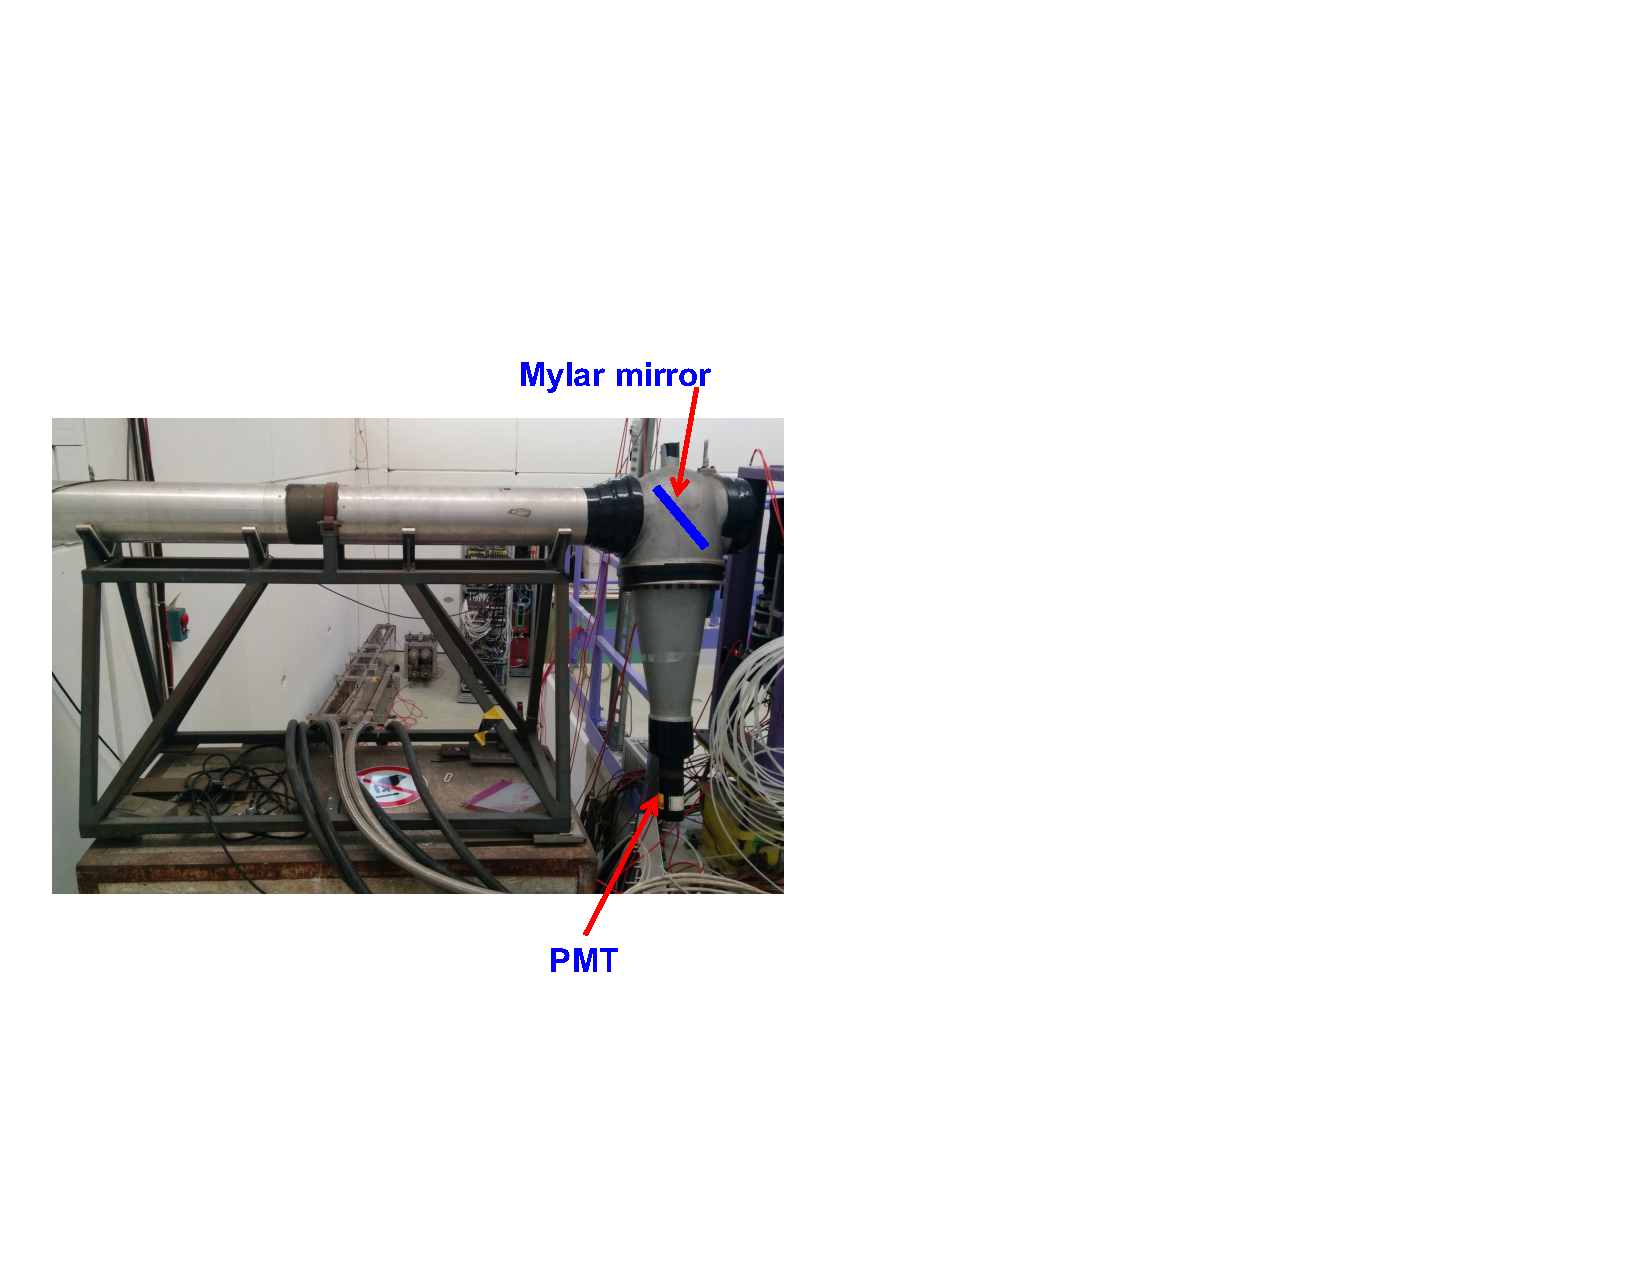
\includegraphics[width=0.65\textwidth]{beamline_ckv.pdf}
\end{cdrfigure}
\begin{cdrfigure}[Cherenkov gases]{ckv_gases}{Gas pressure threshold for the production of Cherenkov light for various particles as a function of particle momentum for Freon 12~\footnote{N. Charitonidis, Y. Karyotakis \it{et al.}, ``Hadron identification proposal for the ProtoDUNE experiments of CENF, to be published.} and CO$_2$ gases.}
  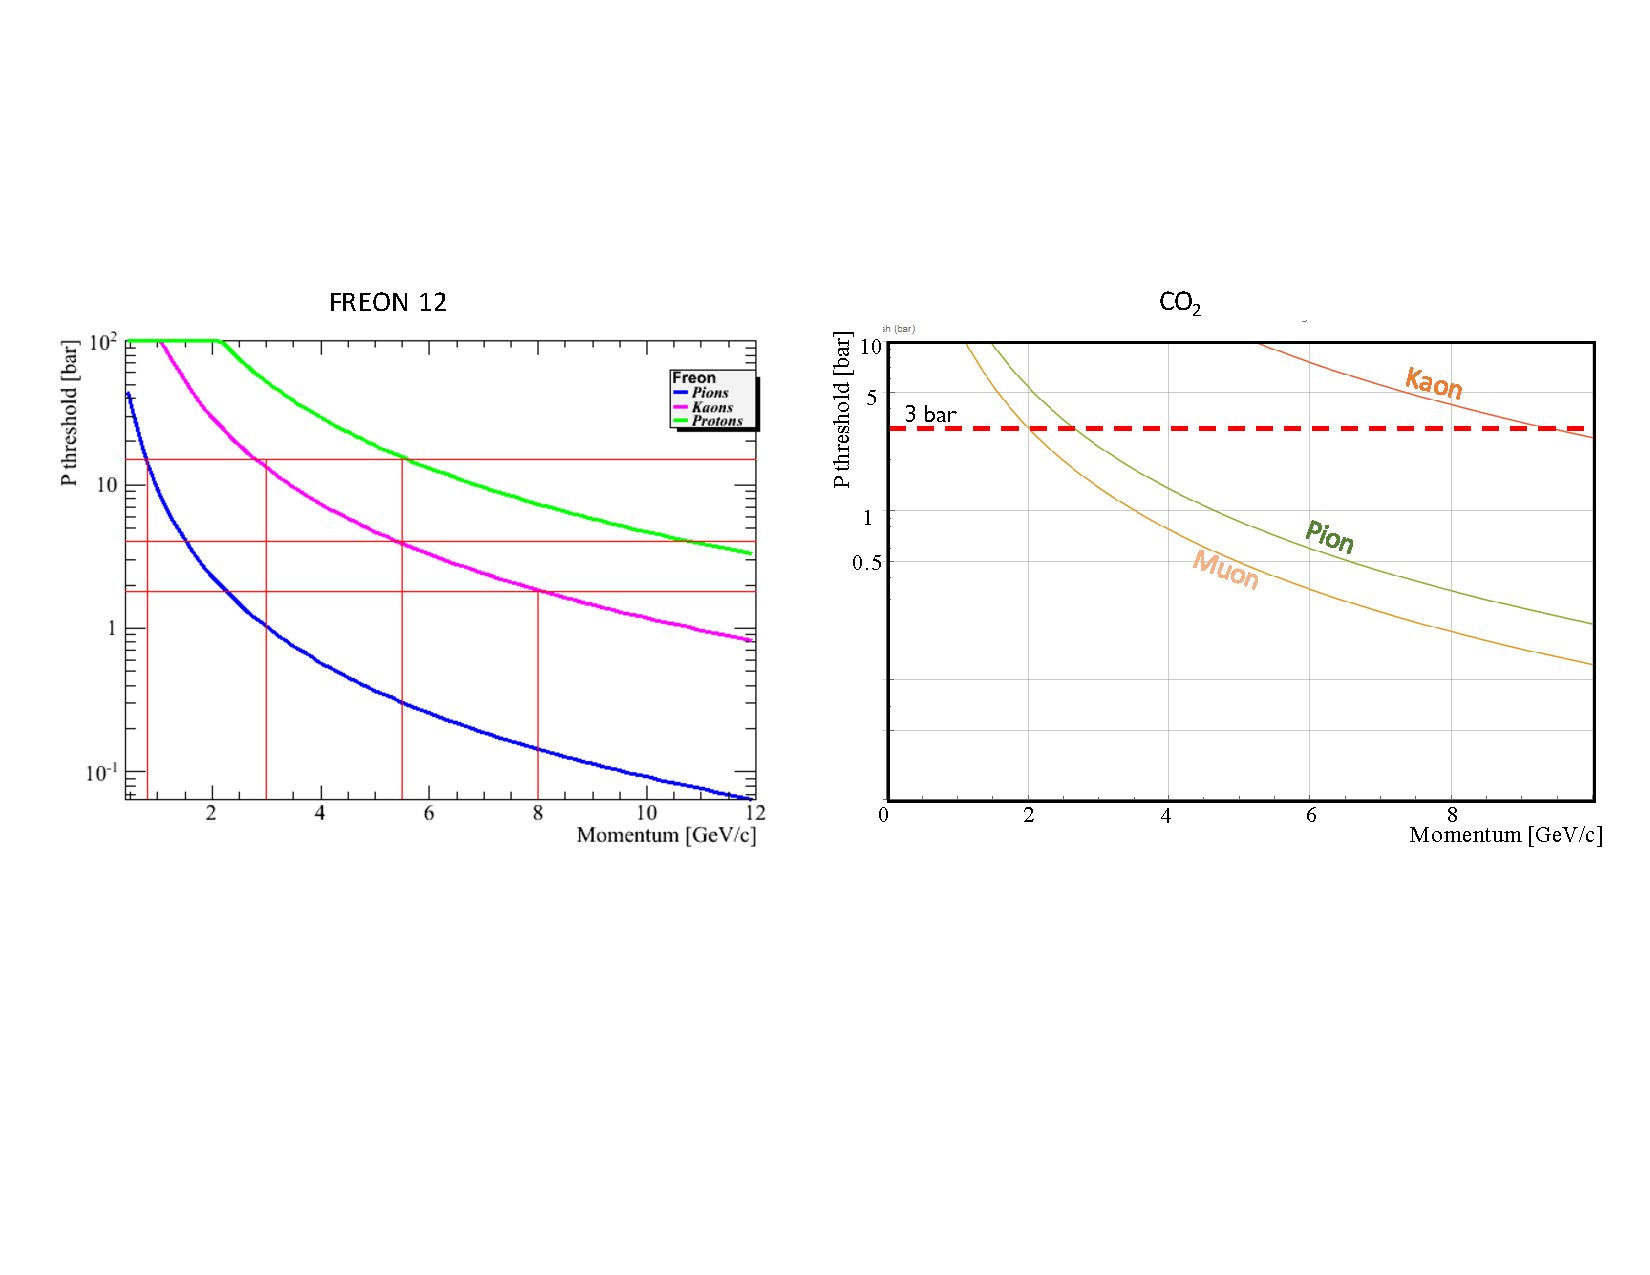
\includegraphics[width=0.99\textwidth]{beamline_CKVgases.pdf}
\end{cdrfigure}
Freon 12 has been selected for its heavier mass, however,  to avoid liquefaction it cannot be operated at pressures larger than 3~bars.  CO$_2$ can be used more easily at higher pressures.  
 Figure~\ref{fig:ckv_gases} shows that pions can be tagged with a 3-bars Freon counter for momenta larger than 2~GeV/c, and kaons can be tagged with a high-pressure  (15-bars) CO$_2$  counter above 4~GeV/c.

The reference plan for beam instrumentation includes a 2-m-long
Cherenkov  counter filled with Freon 12 at adjustable pressure up to
3~bars (XCET1), and a  2-m-long  
 Cherenkov  counter filled with CO$_2$ at adjustable pressure up to
 15~bars (XCET2).
Existing Cherenkov counters at CERN are designed for pressures lower than  3~bar, therefore a new counter has to be manufactured in order to reach the 15~bars needed to efficiently tag kaons. Drawings for such high-pressure Cherenkov counters do exist, as they have been %since they were already 
used in the past. 
Since it will not be necessary to use both counters at all energies, the CO$_2$
counter, filled at low pressure,  will be used for electron discrimination at beam momenta lower
than 4~GeV/c.  

A time-of-flight (ToF) system  is  necessary   to distinguish hadrons below the mentioned thresholds.
%
In summary:
\begin{itemize}
\item {\bf below 2~GeV/c} : one Cherenkov, filled with CO$_2$ at low
  pressure, discriminates electrons; ToF needed for hadrons.
\item {\bf 2-3~GeV/c} : one Cherenkov, filled with CO$_2$ low
  pressure, discriminates electrons; second Cherenkov, filled with
  Freon 12, tags pions; kaons content in this range is very low or negligible.
  ToF is needed to identify protons.
\item {\bf 3-4~GeV/c} : one Cherenkov, filled with CO$_2$ at low
  pressure, discriminates electrons; second  Cherenkov, filled with
  Freon 12, tags pions; ToF is needed for kaon/proton discrimination
\item {\bf 4-7~GeV/c} : one Cherenkov, filled with CO$_2$ at high
  pressure, tags kaons; second  Cherenkov, filled with
  Freon 12, tags pions; electron content of the beam is low and can be
  discriminated by reconstruction.
\end{itemize}

  From table \ref{tab:beampartcomp} it is evident that the kaon content of the beam is negligible at least below 2\,GeV/c, thus  only pion-proton separation is needed at low energies. Figure~\ref{fig:toftau} shows the ToF resolution needed to distinguish among particle species at the $4\sigma$ level as a function of the particle momentum, assuming a 28-m-long path. To distinguish pions from protons below 2\,GeV/c, a 1-ns resolution is enough, while 300~ps are necessary for kaon-proton separation up to  4\,GeV/c. It should also be noted that a ToF system with a $\sim$100-ps resolution would allow identification of protons from other hadrons up to 7\,GeV; this would release the need for a % so that the 
  high-pressure CO$_2$ Cherenkov. %could be avoided. 
  Conversely, covering %in order to cover 
  the full energy range up to 7~GeV for all hadron  types would require a ToF system with a resolution better than 40~ps. % would be needed.
In the following, two (possibly complementary) ToF systems are described.
\begin{cdrfigure}[Required ToF resolution]{toftau}{Required ToF resolution to  distinguish among particle species at the $4\sigma$ level as a function of the particle momentum, assuming a 28-m long path. (The figure shows 23\,m; it needs to be updated.) }
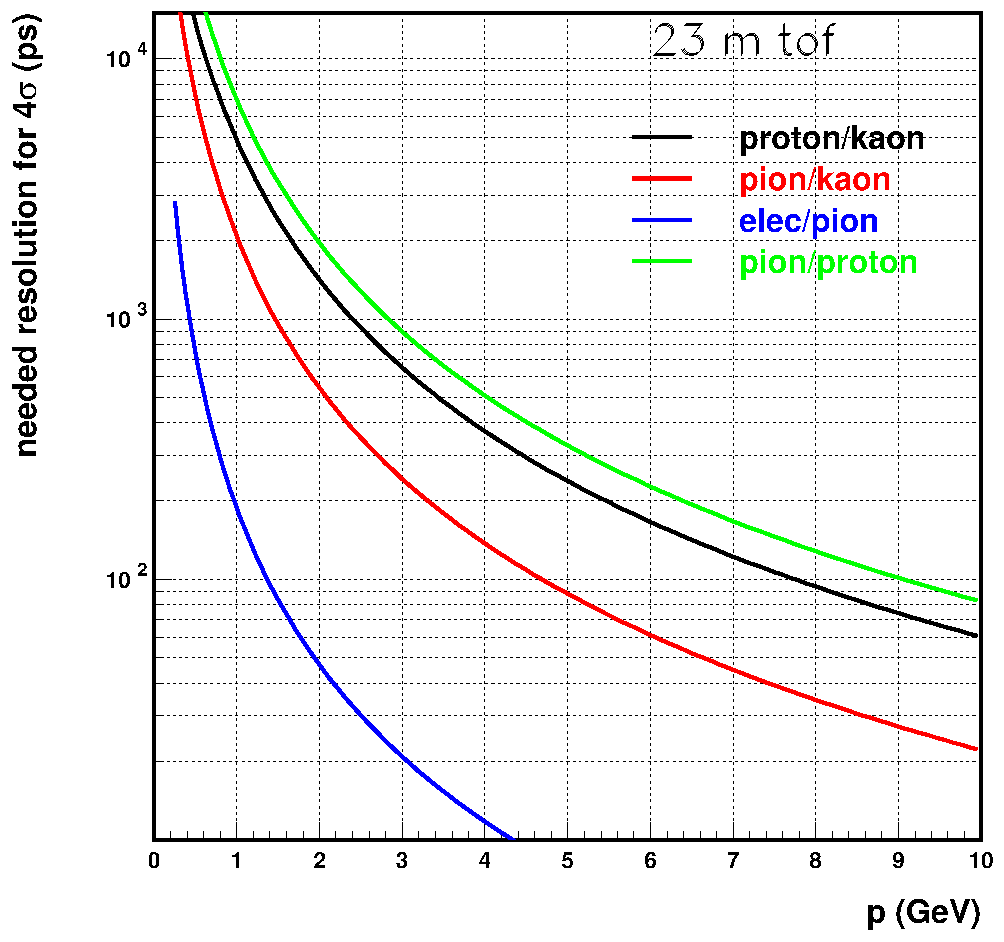
\includegraphics[width=0.65\textwidth]{toftaulow.pdf}
\end{cdrfigure}

\paragraph{pLAPPD time-of-flight system}
Fermilab is testing a ToF system from Argonne National Laboratory that would utilize  
6 $\times$ 6 cm$^2$ prototype
large-area picosecond photodetectors (pLAPPDs), as shown in Figure \ref{fig:pLAPPD}.
 The microchannel plates based devices
are capable of $< 50$ ps resolution with gains of $10^6-10^7$,
mm position resolution along one axis, and slightly worse resolution
along the other axis.  The photodetector is mounted on a readout
board, and the relevant exterior dimensions are 165.1~mm $\times$ 109.3~mm and a
thickness of 16~mm. The active area is defined by the four squares visible in Figure \ref{fig:pLAPPD}, and amounts to about 31~cm$^2$. Tests of these devices in the Fermilab test beam facility (FTBF) are underway, to precisely assess the efficiency and timing capabilities of such a system. 
The pulses from the pLAPPDs will be read out by a fast waveform digitizer and the tests at the FTBF include the development of an artDAQ-based DAQ and potentially a ToF trigger module capable of providing a particle trigger to the ProtoDUNE-SP DAQ.
Larger area pLAPPD can be made to match the H4 beam profile.
\begin{cdrfigure}[pLAPPD  time-of-flight system]{pLAPPD}{Photo of one pLAPPD  time-of-flight device as proposed for the H2 and H4 beamlines.}
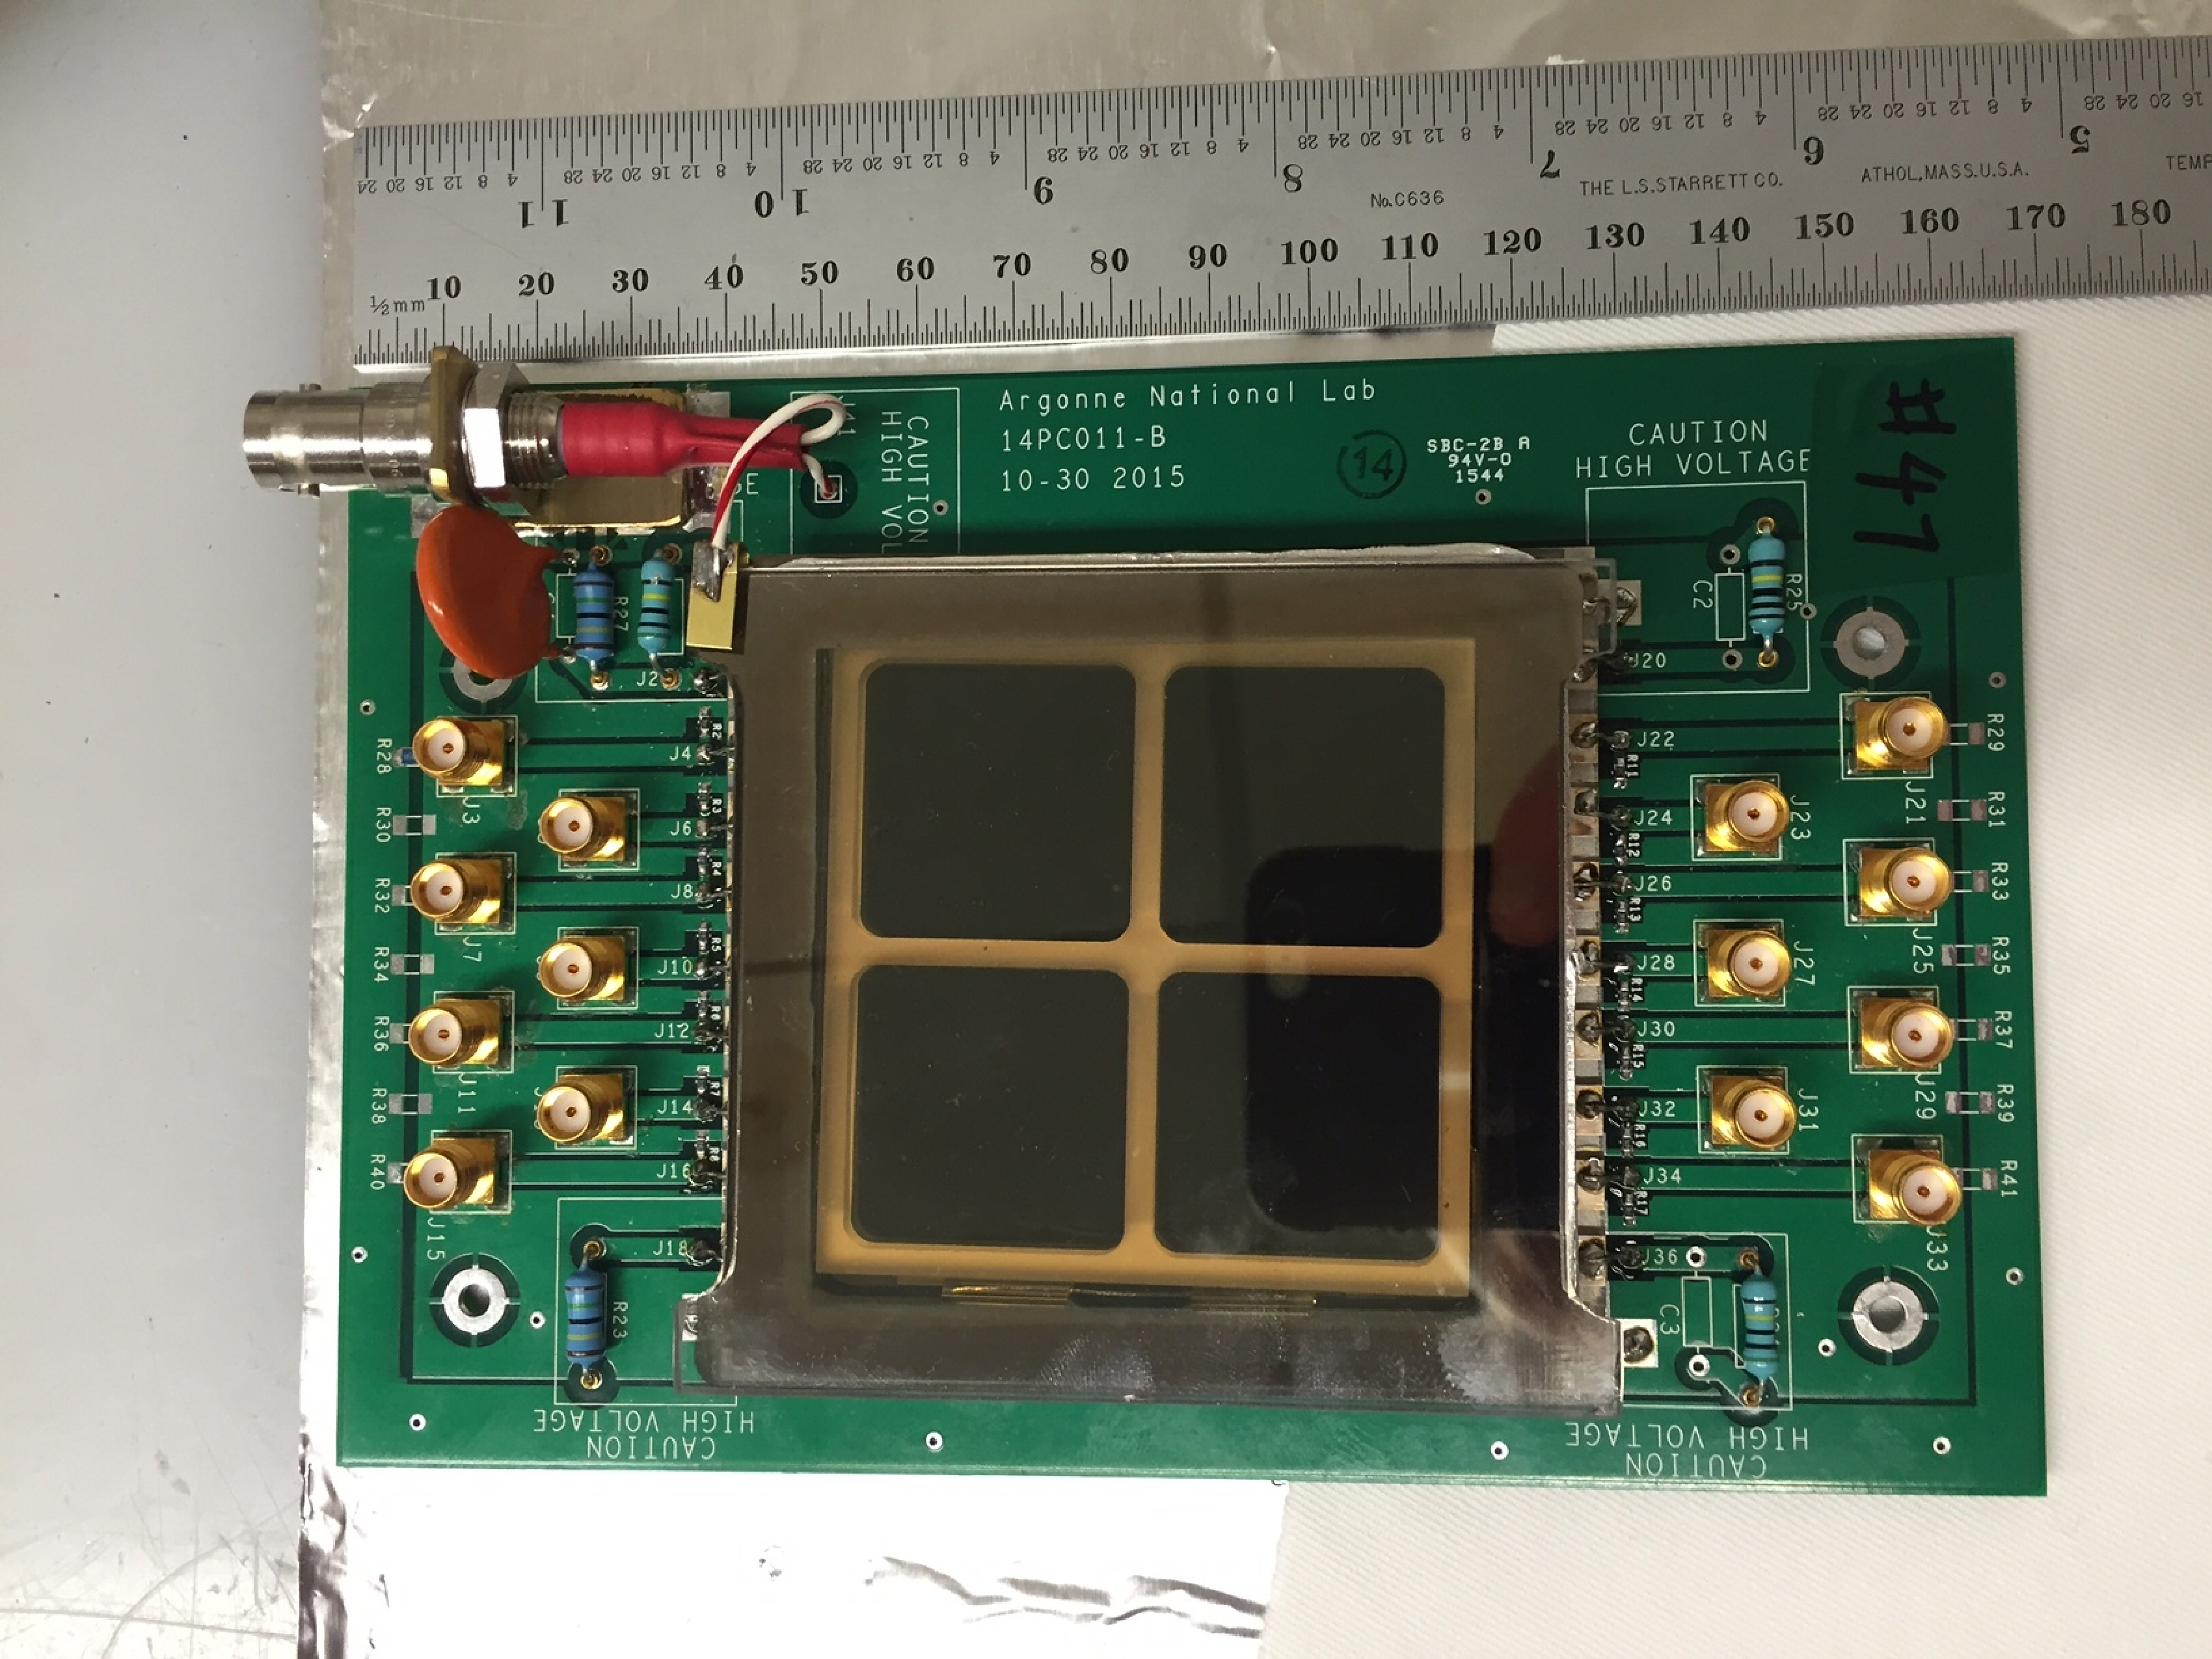
\includegraphics[width=0.65\textwidth]{LAPPD.pdf}
\end{cdrfigure}

\paragraph{Alternative Time-of-flight system}
The  scintillating-fiber monitors can be used also for ToF purposes with the goal of a 1-ns timing resolution, suitable for low momentum ($<$ 2 GeV/c) beams. 
The idea is to read out the detectors with the STiC ASIC~\cite{STIC} (a mixed mode Si photomultiplier readout ASIC for time-of-flight applications) for SiPM readout. 
%%%, developed at the  Kirchhoff Institute for Physics in Heidelberg - will be clear from reference
In this configuration, the time resolution would be dominated by the fiber response. Monte Carlo simulations estimate a resolution better than 1~ns. 
A small prototype will be built and tested in the next few months to fully validate this solution.

%%%%%%%%%%%%%%%%%%%%%%%
\subsection{Material budget and discussion}
\label{beam-material-budget}
The set of beam detectors considered for instrumenting the H4 tertiary beamline include
 five beam monitors (two for tracking and three for spectrometry), two ToF devices, and two high density or pressure gas Cherenkov detectors. The selection of the beam detector configuration in the beamline depends on the type of beam (electron of hadron), and on the beam momentum range. For the electron beam and for low momenta hadron beams the amount of detector material along the beamline may result in particle energy degradation and significant reduction of the beam rate delivered at the active detector due to scattering outside the beam pipe. A FLUKA\cite{Ferrari:2005zk,Fluka15} 
 simulation was used to evaluate these effects accounting for the 
 detector materials in the beamline, and materials of the beam window, cryostat and beam plug. Figure~\ref{fig:matblfull} shows the cumulative increase of the material budget along the tertiary beam line from the target to the TPC, expressed in terms of fraction of radiation length (red line - total  $0.6X_0$) and of interaction length (black line - total  $0.15 \lambda_I$). The average energy loss for a mip is about 28~MeV.
 The largest contribution to the energy-loss and energy degradation is due to the high pressure Cherenkov detectors and to the pLAPPD. Except for a low-pressure Cherenkov counter for electron discrimination, the high pressure Cherenkov are not necessary at low hadron beam momenta  and can be removed or just emptied. Scintillating fiber beam monitors can replace the pLAPPD as ToF devices for the lowest-momentum beam. 

  
 \begin{cdrfigure}[Material budget]{matblfull}{Material budget in the beamline, as a function of the distance from the center of the detector (in cm). The red line describes the amount of $X_0$, the black line the amount of interaction length, both read on the left axis. The black dotted line is the average energy lost by a mip particle, and is read on the right axis (in MeV). Vertical lines show the positions of the various beam monitors (in between the two blue lines are the 3 devices for spectrometry, ``bm'' is the last beam monitor, ``bw'' is the starting point of the beam window).}  
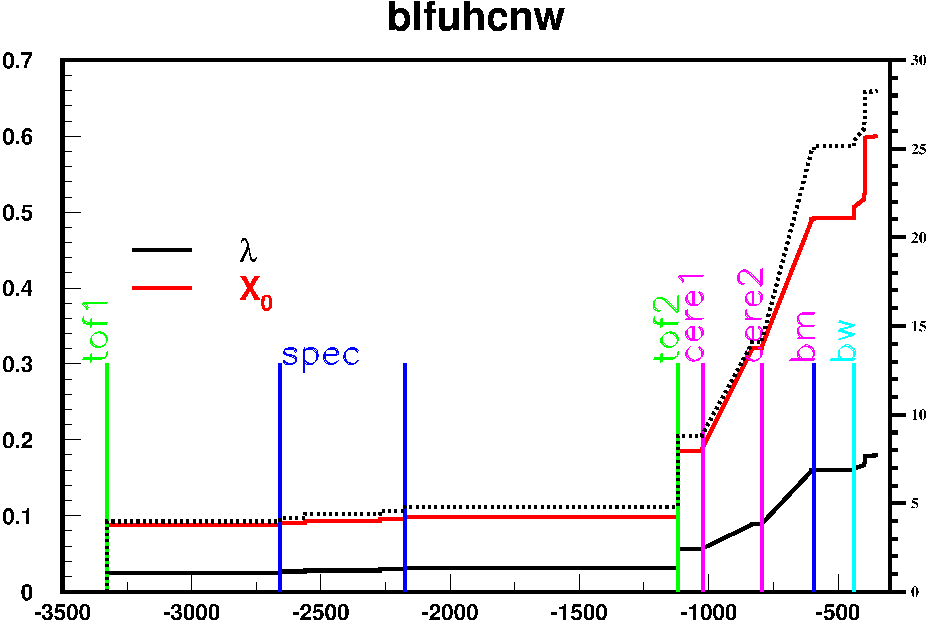
\includegraphics[width=0.65\textwidth]{blfuhcnwrayplo.pdf}
\end{cdrfigure}
 
 Scattering of low-energy pions and protons in crossing the detector material significantly reduces their content in the low-momenta hadron beam reaching the detector active volume. For example, at 1~GeV/c the rate of pions arriving at the detector is reduced by a factor of 2.5, and the rate of protons 
 is reduced by a factor of 4. 


%%%%%%%%%%%%%%%%%%%%%%%
\subsection {Trigger and data acquisition}

The beam instrumentation can provide a trigger signal, built from the coincidence of the two last beam monitors, vetoed by the electron-tagging Cherenkov for low-energy beams. 
A trigger mask, providing the status of the other counters, can also be provided. 
 Synchronization of the detector data acquisition (DAQ) with the beam instrumentation DAQ will be ensured by a common time stamp through a White Rabbit network.

Beam instrumentation data will be read out independently on a separate DAQ stream. However,  
the beam data fragments corresponding to  events with a valid trigger from both beam and ProtoDUNE-SP will be merged online with the detector data.
 
